\section{Lightweight State-of-the-Art Models}
\subsection{MobileNetV2}
MobileNetV2 uses inverted residual blocks and linear bottlenecks
\cite{sandler2018}. We load torchvision's explicit ImageNet
\texttt{IMAGENET1K\_V2} weights and replace its classifier with a ten-class head.
Its depthwise layers reduce spatial filtering cost, while pointwise expansion
and projection layers mix channels. It is still much larger than Model B:
``lightweight'' does not imply compliance with the custom parameter limit.
\subsection{EfficientNet-B0}
EfficientNet balances network depth, width and resolution \cite{tan2019}.
We use torchvision's B0 \texttt{IMAGENET1K\_V1} weights and replace its final
classifier. No fallback to random initialization is permitted.
It retains inverted bottlenecks, squeeze-and-excitation channel weighting
and its original nonlinearities. The pretrained comparison includes prior
ImageNet learning as well as architectural differences.
\subsection{Transfer Learning Strategy}
Stage one trains the head for two epochs using Adam at 0.001; feature weights
and feature batch-normalization running statistics remain frozen. Stage two
unfreezes the entire network and uses a new Adam optimizer at 0.0001 for eight
epochs. Validation selects the checkpoint across both stages. Both models use
exactly the saved custom-model split and the same 64x64 preprocessing.
Table~\ref{tab:transfer_stages} distinguishes trainable counts and timing in
the frozen-head and full-network stages. Both use the shared training loop.
% Generated from saved experiment evidence; do not edit values.
\begin{table}[H]\centering\small
\caption{Transfer-learning stages, learning rates and measured mean epoch times.}\label{tab:transfer_stages}
\begin{tabular}{lrrrrr}
\toprule
Model & Stage & Epochs & LR & Trainable & Epoch (s) \\ \midrule
MobileNetV2 & head & 2 & 0.001 & 12,810 & 3.347 \\
MobileNetV2 & finetune & 8 & 0.0001 & 2,236,682 & 7.915 \\
EfficientNet-B0 & head & 2 & 0.001 & 12,810 & 4.263 \\
EfficientNet-B0 & finetune & 8 & 0.0001 & 4,020,358 & 11.175 \\
\bottomrule
\end{tabular}
\end{table}

\subsection{Results}
Table~\ref{tab:pretrained_accuracy} reports classification metrics, while
Table~\ref{tab:pretrained_resources} separates total and fine-tuning trainable
parameters, checkpoint size and epoch time. MobileNetV2 is
\TransferAccuracyGap{} percentage points more accurate than EfficientNet-B0
in this run despite having fewer parameters. A larger pretrained model does
not automatically give a better result at this input size and training budget.
% Generated from saved experiment evidence; do not edit values.
\begin{table}[H]\centering\small
\caption{Held-out test metrics for pretrained models; P is precision and R is recall.}\label{tab:pretrained_accuracy}
\begin{tabular}{lrrr}
\toprule
Model & Accuracy (\%) & Macro P (\%) & Macro R (\%) \\ \midrule
MobileNetV2 & 97.31 & 97.20 & 97.21 \\
EfficientNet-B0 & 96.81 & 96.72 & 96.71 \\
\bottomrule
\end{tabular}
\end{table}

% Generated from saved experiment evidence; do not edit values.
\begin{table}[H]\centering\small
\caption{Pretrained-model resources. Trainable counts refer to fine-tuning; timing averages both stages.}\label{tab:pretrained_resources}
\begin{tabular}{lrrrr}
\toprule
Model & Total & Trainable & Size (MiB) & Epoch (s) \\ \midrule
MobileNetV2 & 2,236,682 & 2,236,682 & 8.754 & 7.002 \\
EfficientNet-B0 & 4,020,358 & 4,020,358 & 15.604 & 9.793 \\
\bottomrule
\end{tabular}
\end{table}

Figure~\ref{fig:mobilenet_v2_curves} shows improvement from
\MobileHeadVal\% validation accuracy after head training to a best of
\MobileBestVal\% at epoch \MobileBestEpoch{}, a gain of
\MobileFineGain{} percentage points. Updating the features is therefore
useful under this schedule. Training loss increases at the first fine-tuning
epoch, coinciding with unfreezing and switching the feature extractor to
training mode. Feature batch-normalization statistics are then updated;
EfficientNet-B0 also activates stochastic depth in its feature extractor.
These changed training conditions must be considered when reading the
stage-transition losses.
\begin{figure}[H]\centering
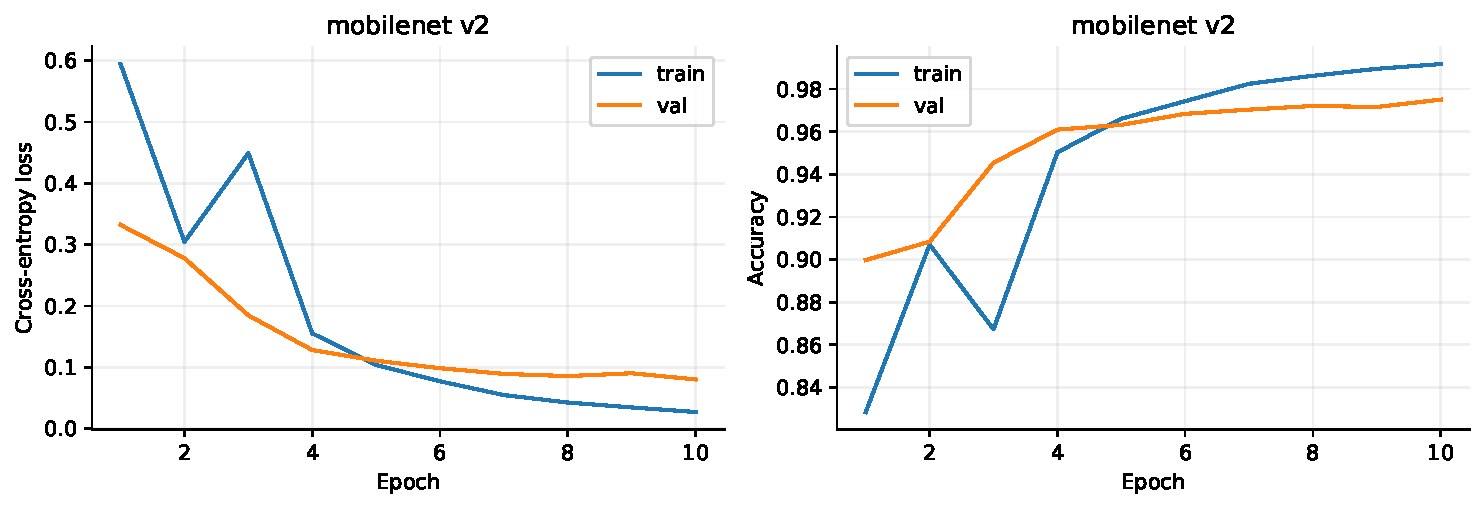
\includegraphics[width=0.96\textwidth]{figures/mobilenet_v2_curves.pdf}
\caption{MobileNetV2: frozen-head epochs 1--2 and full-network fine-tuning epochs 3--10.}
\label{fig:mobilenet_v2_curves}
\end{figure}
\begin{figure}[H]\centering
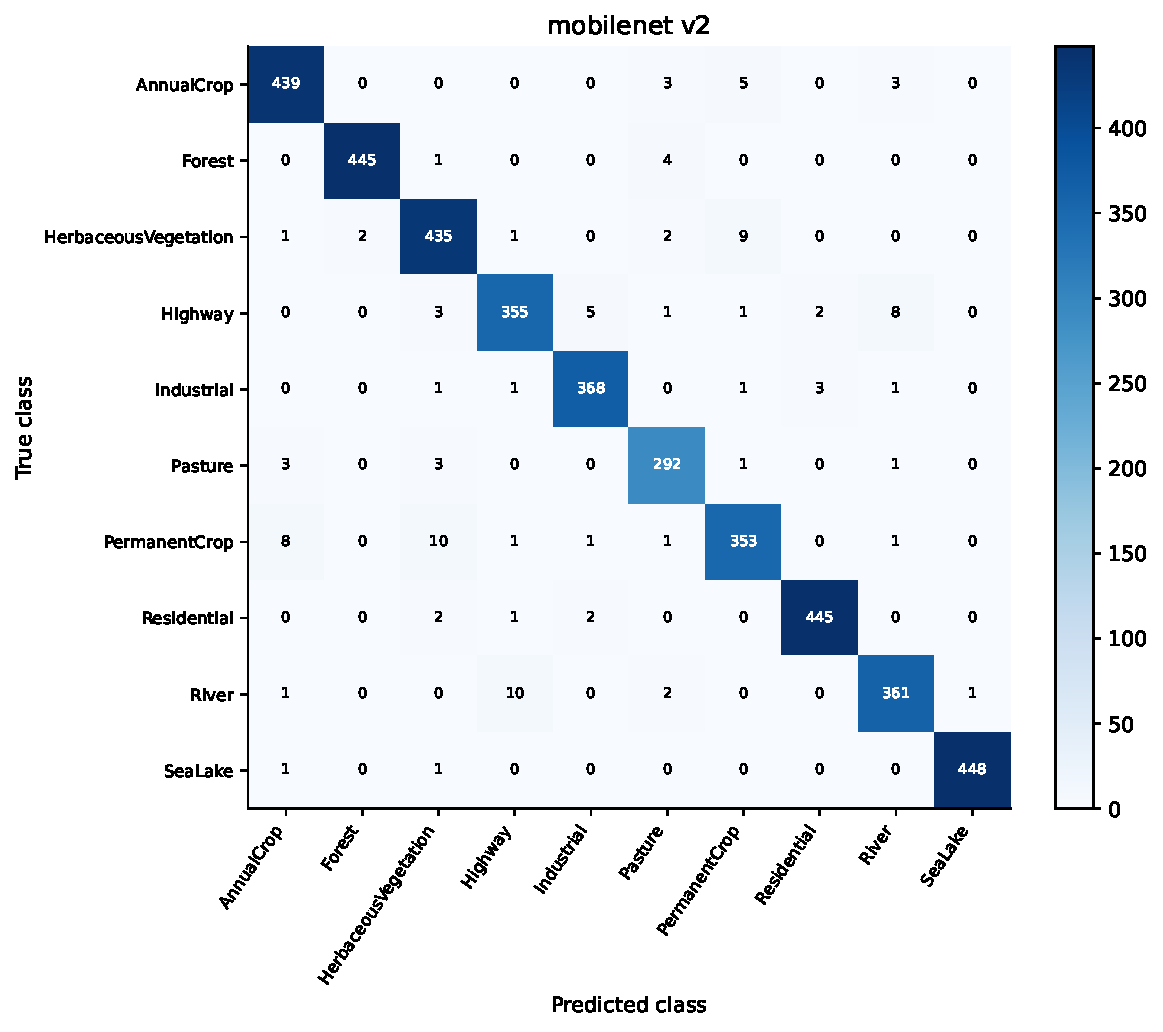
\includegraphics[width=.72\textwidth]{figures/mobilenet_v2.pdf}
\caption{MobileNetV2 test confusion matrix (counts).}
\label{fig:mobilenet_v2_cm}
\end{figure}
Figure~\ref{fig:mobilenet_v2_cm} shows MobileNetV2's remaining class errors;
Section~\ref{sec:discussion} examines the largest directed confusions.
EfficientNet-B0 improves from \EfficientHeadVal\% validation accuracy after
head training to \EfficientBestVal\% at epoch \EfficientBestEpoch{}, a gain
of \EfficientFineGain{} percentage points.
Figure~\ref{fig:efficientnet_b0_curves} shows the same stage-transition
training-loss increase, followed by improvement. Training loss continues to
fall late in the run while validation performance levels off, so its selected
checkpoint precedes the final epoch. Figure~\ref{fig:efficientnet_b0_cm}
shows its test errors, including confusion between crop classes.
\begin{figure}[H]\centering
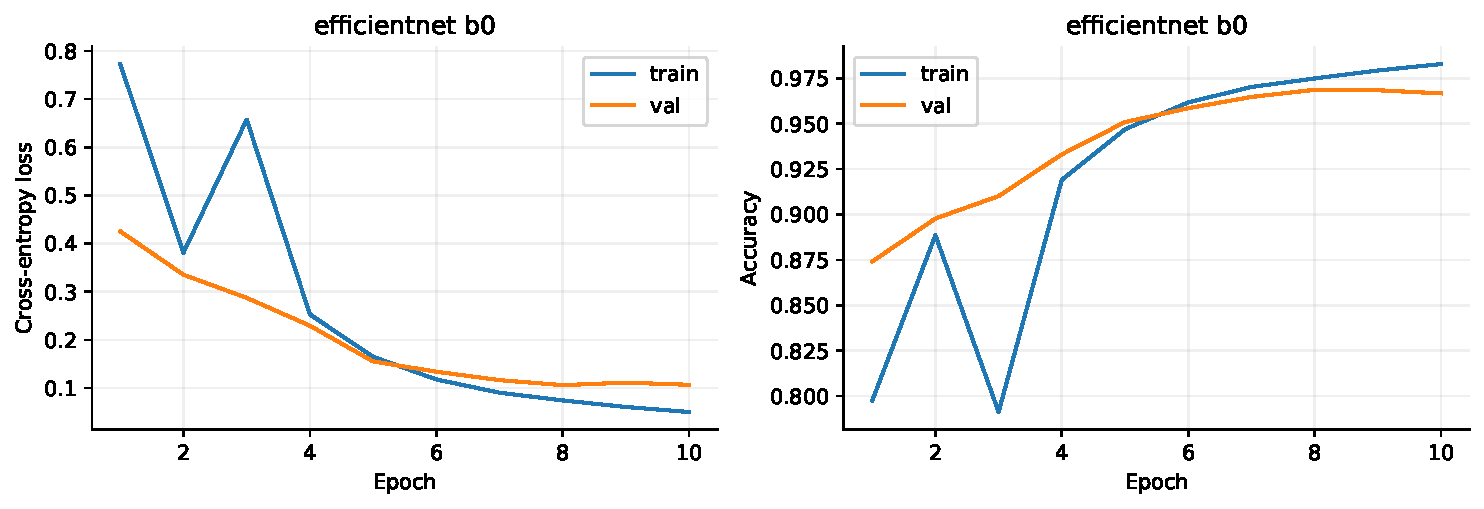
\includegraphics[width=0.96\textwidth]{figures/efficientnet_b0_curves.pdf}
\caption{EfficientNet-B0: frozen-head epochs 1--2 and full-network fine-tuning epochs 3--10.}
\label{fig:efficientnet_b0_curves}
\end{figure}
\begin{figure}[H]\centering
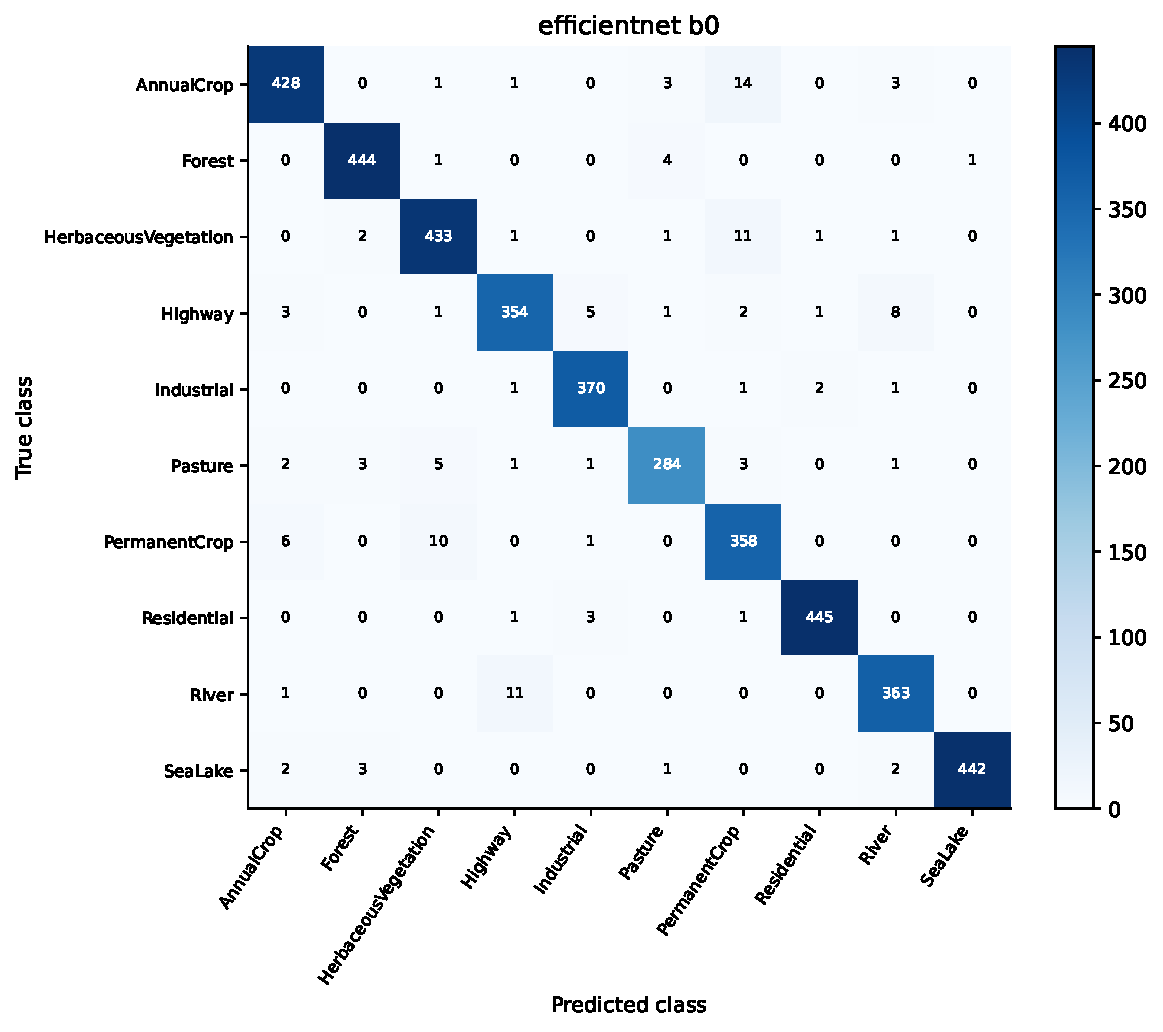
\includegraphics[width=.72\textwidth]{figures/efficientnet_b0.pdf}
\caption{EfficientNet-B0 test confusion matrix (counts).}
\label{fig:efficientnet_b0_cm}
\end{figure}
